\section*{Problem 4}

\begin{enumerate}
	\item From the correlation matrix it looks like displacement, weight, and horsepower all have a high positive correlation with cylinders. Given what we know about cars this makes intuitive sense. Horsepower is most positively correlated with displacement and mpg is most negatively correlated with weight, which, again, makes intuitive sense. 
	\item The scatter plots for three highly correlated variables are below. 
	\newline
	\begin{figure}[htbp]
		\centering
		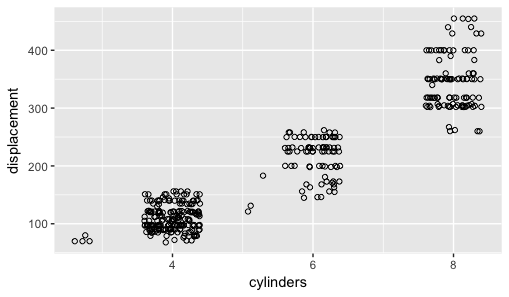
\includegraphics[width=.8\linewidth]{img/ESL_02_disp_vs_cyl.png}
	\end{figure}
	\begin{figure}[htbp]
		\centering
		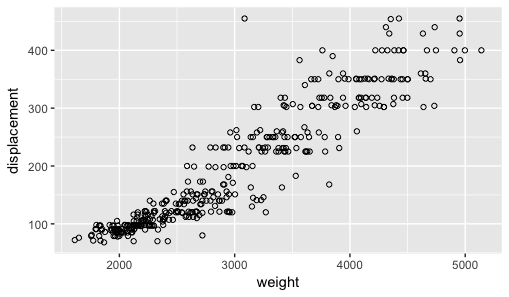
\includegraphics[width=.8\linewidth]{img/ESL_02_disp_vs_weight.png}
	\end{figure}
	\begin{figure}[htbp]
		\centering
		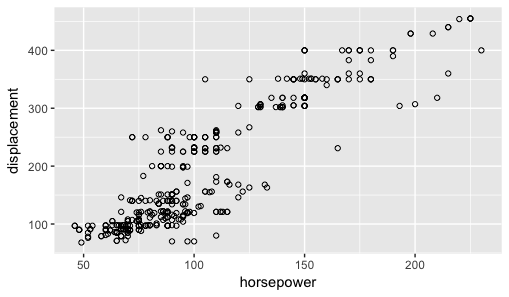
\includegraphics[width=.8\linewidth]{img/ESL_02_disp_vs_horsepower.png}
	\end{figure}
	\newpage
	Scatterplots for three highly anti-correlated variables are below.
	\begin{figure}[htbp]
		\centering
		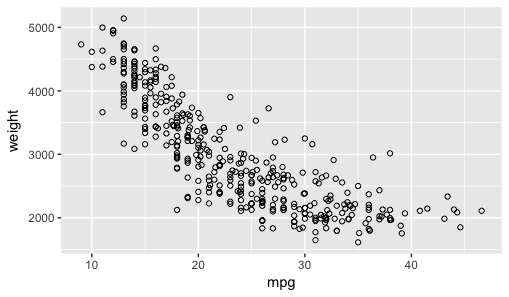
\includegraphics[width=.8\linewidth]{img/ESL_02_weight_vs_mpg.png}
	\end{figure}
	\begin{figure}[htbp]
		\centering
		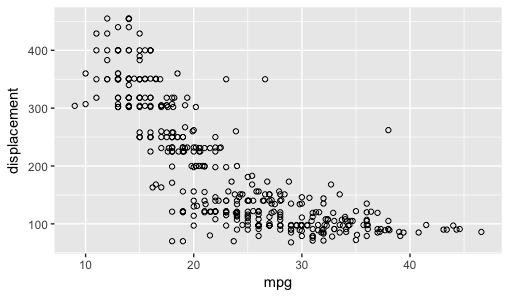
\includegraphics[width=.8\linewidth]{img/ESL_02_disp_vs_mpg.png}
	\end{figure}
	\begin{figure}[htbp]
		\centering
		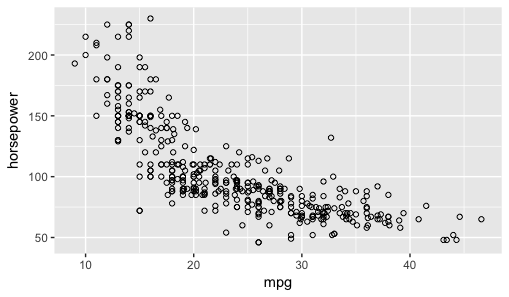
\includegraphics[width=.8\linewidth]{img/ESL_02_hrsp_mpg.png}
	\end{figure}
	\newpage
	The number of cylinders, the weight of the vehicle, and the horsepower have the highest correlations with displacement, respectively. Some of these numbers make intuitive sense from what we know about how internal combustion engines work. If you want more displacement adding more cylinders is one option to achieve this. Weight, displacement and horsepower are also highly anti-correlated with mpg. So, as the vehicle gets heavier, or gets an increase in power, the efficiency of the engine reduces and you get fewer miles per gallon.
	\newpage
	\item  The p-values show that all of the predictors have a statistically significant relationship to the outcome. From the $R^2$ values displacement as a predictor is a more accurate model. Also, year as a predictor is the least accurate model.  
	\newline
	\begin{tabular}{ccc}
		\centering
		Run Type & $R^2$ & p-value \\
		\hline
		mpg ~ cyl & $0.6047$ & \\
		mpg ~ disp & $0.6482$ &  \\
		mpg ~ hrsp & $0.6059$ &  \\
		mpg ~ year & $0.337$ &
	\end{tabular}
	\item The $R^2$ is 0.8125, which is close to 1. This suggests that this model is an accurate model. Cylinders and horsepower were both statistically significant predictor alone, but in multivariate regression they are not. The coefficients describe the size of the effect of the predictor on the response variable, therefore a negative coefficient gives the amount of decrease in the response for every increase in the predictor.
	\item The residual plot does suggest a non-linearity in the data. The far left side of the plot shows consistent over prediction (i.e. bias) in the data. There don't seem to be any unusually large outliers. There is a high leverage point, point at index 14, as seen in the image below. 
	\begin{figure}[htbp]
		\centering
		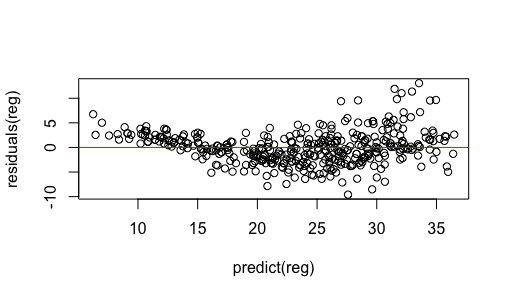
\includegraphics[width=.8\linewidth]{img/ESL_02_nonlinearity.png}
	\end{figure}
	\begin{figure}[htbp]
		\centering
		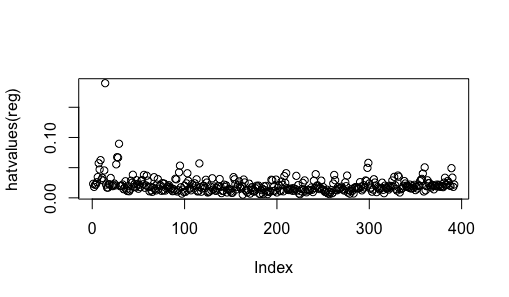
\includegraphics[width=.8\linewidth]{img/ESL_02_leverage.png}
	\end{figure}
	
	\item The transformations with other variables like weight, year or cylinder improve the result ($R^2$ value) but transforming displacement with itself does not make the model better. Doing transformations on one predictor doesn't give you as much benefits as using more predictors. 
	
\end{enumerate}  


